\subsection{Trigger formulations and the accuracy of the affine rule}

Table~\ref{tab:formulations} lists the affine rule and three alternative trigger formulations. All except the equilibrium of \citet{HuangYu2021} are evaluated numerically. The pre-commitment $\aMEU$ optimum serves as the accuracy benchmark. The recursive $\alpha$-mixture of the generator serves as an analytical comparator. Here, $\Vlin(\alpha)$ denotes the member trigger of Eq.~(\ref{eq:affine}), and $\VMEU(\alpha,V_0)$ denotes the benchmark optimum at the same recorded weight.

\subsubsection{The pre-commitment benchmark}

For a trigger $V^{*}$ and a reference project value $V_0<V^{*}$, let $\tau$ denote the first hitting time of $V^{*}$. The standard real-options expression gives
\begin{equation}
\mathbb{E}_{\sigma}\bigl[e^{-r\tau}(V_{\tau}-I)\bigr]=\Bigl(\frac{V_0}{V^{*}}\Bigr)^{\beta_1(\sigma)}(V^{*}-I).
\label{eq:hitting}
\end{equation}
At this step, the ambiguity set is the pair of constant-volatility measures indexed by the declared endpoints. The factor $(V_0/V^{*})^{\beta_1}$ decreases in $\beta_1$ when $V_0<V^{*}$, and $\beta_1(\sigma)$ decreases in $\sigma$. The infimum and supremum of Eq.~(\ref{eq:hitting}) over the set are therefore attained at $\slow$ and $\shigh$, respectively. No admissible calibration reverses this endpoint ordering. A reversal would require a reference value above the trigger, or an exercise payoff whose value decreases in volatility. The $\aMEU$ objective for a trigger rule is
\begin{multline}
J^{\alpha}(V^{*},V_0)=(V^{*}-I)\\
\times\biggl[\alpha\Bigl(\frac{V_0}{V^{*}}\Bigr)^{\beta_1(\slow)}+(1-\alpha)\Bigl(\frac{V_0}{V^{*}}\Bigr)^{\beta_1(\shigh)}\biggr].
\label{eq:Jalpha}
\end{multline}
The optimal trigger $\VMEU(\alpha,V_0)\equiv\arg\max_{V^{*}}J^{\alpha}(V^{*},V_0)$ has no closed form for $\alpha\in(0,1)$. Bounded scalar optimization computes it. Solving this scalar problem at each recorded weight yields the benchmark member-threshold vector. The maximization runs over constant triggers. The solution is therefore optimal within the class of constant-threshold rules under the pre-commitment criterion.

Unlike the affine rule, the benchmark vector depends on the reference project value $V_0$. The pre-commitment objective is evaluated directly at this value, without a recursive value function. The benchmark is defined for $V_0$ below the benchmark trigger of every member, a region called the benchmark domain. We fix $V_0=I$, the value at which immediate investment just breaks even. This value lay in the domain at every evaluated cell. A cell entered the evaluation only when $V_0$ lay below the low-endpoint trigger $\Vlow$. By Proposition~\ref{prop:benchmark}(i), this is a conservative sufficient form of the domain condition. Both calculations use the same economic primitives, volatility endpoints, recorded weights, and radius grid.

Table~\ref{tab:formulations} arranges the four formulations by role. The recursive $\alpha$-mixture shares two features with the affine rule, a closed form and independence from the reference value. The benchmark serves as the comparator at the same reporting granularity, a member-indexed threshold vector. It is required whenever the affine-only release rule fails. The equilibrium of \citet{HuangYu2021} completes the table.

Two conditions qualify the benchmark vector as the accuracy standard. The computed maximizer must be global, and its position relative to the affine trigger must be known. Proposition~\ref{prop:benchmark} settles both through one quantity, the spread between the two endpoint exponents.

\begin{proposition}[Benchmark well-posedness and one-sidedness]\label{prop:benchmark}
Write $\blo:=\beta_1(\slow)$ and $\bhi:=\beta_1(\shigh)$ for the exponents at the two endpoints, and $\Db:=\blo-\bhi>0$ for their spread. Fix a recorded weight $\alpha$ and a reference project value $V_0$ in the benchmark domain.
\begin{enumerate}
\item[(i)] Unique global maximizer. Every stationary point of $J^{\alpha}$ lies in $[\Vlow,\Vhigh]$. If
\begin{equation}
\Db\le 1\quad\text{or}\quad(\Db-1)\,\Vhigh\le\Db\,\Vlow,
\label{eq:unique}
\end{equation}
the stationary point is unique and is the global maximizer. Condition~(\ref{eq:unique}) is free of $\alpha$ and of $V_0$.
\item[(ii)] One-sidedness. Assume Condition~(\ref{eq:unique}). For $\alpha\in(0,1)$,
\begin{equation}
\Vlin(\alpha)\ge\VMEU(\alpha,V_0)\iff\frac{\blo-1}{\bhi-1}\ge\Bigl(\frac{\Vlin(\alpha)}{V_0}\Bigr)^{\Db}.
\label{eq:onesided}
\end{equation}
The affine and benchmark triggers coincide at the endpoint weights $\alpha=0$ and $\alpha=1$. Since $\Vlin$ decreases in $\alpha$, replacing it by $\Vhigh$ yields a condition sufficient for every recorded weight at once. At $V_0=I$, the condition holds whenever $\Db\le1$.
\end{enumerate}
\end{proposition}

Both conditions have closed forms in the calibration and the radius. A gate can therefore check them without solving the benchmark. Condition~(\ref{eq:unique}) held at all 33 admissible calibrations across the admissible radius range, with a slack of at least $0.906I$. The global-maximizer property therefore held for every reported benchmark value. A separate scan covered 30,090 cells defined by calibration, radius, reference value, and weight. It counted exactly one interior maximum of $J^{\alpha}$ in every cell. The same counter flagged a deliberately bimodal control function. Condition~(\ref{eq:onesided}) held at all 33 calibrations and every registered radius up to 22\%. At the 33\% stress radius, it failed at one calibration, with $r=0.12$, $\mu_c=0.02$, and $\sbar=0.199$. There, the affine trigger fell below the benchmark for recorded weights near 0.01. The relative gap was at most $4.5\times10^{-6}$, confirmed at 40-digit precision. This failure lies above the 10\% cap, where the release rule already requires a dual report.

\begin{table*}[!t]
\caption{Decision-rule outputs and their roles in this paper.}
\label{tab:formulations}
\centering
\footnotesize
\renewcommand{\arraystretch}{1.15}
\begin{tabular}{@{}L{0.17\textwidth}L{0.25\textwidth}L{0.14\textwidth}L{0.36\textwidth}@{}}
\toprule
Formulation & Type of output & Dynamic consistency & Role in this paper\\
\midrule
Affine endpoint rule, Eq.~(\ref{eq:affine}) & Member-trigger map $\alpha_i\mapsto V^{*}_{i}(t)$. Eqs.~(\ref{eq:price}) and (\ref{eq:interval}) convert it to $\{P^{*}_{i}\}$, $C_t$, and $B_t$ & Not applicable (static gate-reporting map) & Closed-form mechanism, independent of the reference value, preserving member thresholds\\
Pre-commitment $\aMEU$ optimum, Eq.~(\ref{eq:Jalpha}) & Member-trigger vector dependent on $V_0$, evaluated at $\{\alpha_i\}$ & No (pre-commitment rule) & Direct comparator, benchmark available by recomputation at any gate, and required fallback\\
Recursive $\alpha$-mixture of the generator, Eq.~(\ref{eq:effvar}) & Member-trigger vector $V^{*}(\sigma_{\mathrm{eff}}(\alpha_i))$, independent of $V_0$, with a unique scalar boundary & Yes, by construction & Third comparator. Its critical weight has the closed form of Eq.~(\ref{eq:critrec}) and lies above one half. The variance mixture fixes this value for any increasing trigger map\\
Time-consistent $\aMEU$ equilibrium \citep{HuangYu2021} & Member-indexed equilibrium stopping regions. Scalar boundaries apply only when uniquely defined in a common state & Yes & On the constant-endpoint set of this paper, the recursive row is time-consistent with a single-threshold stopping region, as a threshold report requires. Under state-dependent prior sets, compressing the regions into $\{P^{*}_{i}\}$ is inadmissible\\
\bottomrule
\end{tabular}
\end{table*}

\subsubsection{The recursive alternative}

The pre-commitment objective is evaluated once, at the gate. Applying the same $\alpha$-mixture at every state yields a rule dynamically consistent by construction. In this setting, the rule also has a closed form. Under convexity of the continuation value, the generator collapses to the ordinary geometric Brownian form at the effective variance
\begin{equation}
\sigma^{2}_{\mathrm{eff}}(\alpha)=\alpha\,\slow^{2}+(1-\alpha)\,\shigh^{2}.
\label{eq:effvar}
\end{equation}
The recursive trigger is then $V^{*}_{\mathrm{rec}}(\alpha)=V^{*}(\sigma_{\mathrm{eff}}(\alpha))$. It is free of any reference project value. Solving $\sigma_{\mathrm{eff}}(\tilde{\alpha})=\sbar$ gives the critical weight
\begin{equation}
\tilde{\alpha}_{\mathrm{rec}}(h)=\frac{1}{2}+\frac{h}{4\sbar},
\label{eq:critrec}
\end{equation}
which exceeds one half at every positive radius.

Convexity also makes the effective variance state-independent, so the recursive problem reduces to the ordinary stopping problem at this variance. Its stopping region is bounded by a single threshold. A time-consistent formulation thus meets the reporting condition in this setting. The recursive columns of Table~\ref{tab:threeform} report the implied critical weight and interval width. The recursive rule remains a comparator for one reason. Mixing the two generators mixes variances, so a recorded weight indexes an effective volatility. Under the affine rule, the weight indexes a position between the two endpoint triggers.

Eqs.~(\ref{eq:critrec}) and (\ref{eq:kappa}) locate the difference between the two rules. The recursive displacement is $h/(4\sbar)$. Its coefficient of $h$ equals the geometric term of the curvature ratio. The affine coefficient also retains a negative $\beta$-curvature correction. Near the anchor, the affine critical weight therefore lies below the recursive one. Table~\ref{tab:threeform} compares all three formulations, and this ordering held at every evaluated radius. The affine and recursive critical weights lay above one half. The pre-commitment critical weight at $V_0=I$ lay below one half and decreased in the radius. Under the benchmark at this reference value, both the sign of Corollary~\ref{cor:global} and the monotonicity of Corollary~\ref{cor:mono} reverse. At the baseline calibration and the four-member reference profile, the widths differed far less than the labels. At a 10\% radius, the widths were 10.945\,CNY/t (affine), 11.027\,CNY/t (recursive), and 10.717\,CNY/t (pre-commitment). The two comparators lay within 2.1\% of the affine width. This distance grew with the radius and reached 6.4\% at the 33\% stress radius. This magnitude was close to the 6.15\% maximum trigger error over all calibrations and the full radius grid.

The closed forms in Eqs.~(\ref{eq:critical}) and (\ref{eq:critrec}) both rest on the perpetual geometric Brownian structure. Eq.~(\ref{eq:critrec}) requires a convex continuation value, so the generator collapses to Eq.~(\ref{eq:effvar}). The displacement in Eq.~(\ref{eq:critical}) requires $V^{*}(\sigma_p)$ to be convex in $\sigma_p$. A different price process can break either property. The ratio in Eq.~(\ref{eq:critical}) was therefore recomputed under three further specifications. These were a finite investment horizon, a mean-reverting log price, and a jump diffusion. Each specification is solved on one grid shared by the three volatility endpoints. The discretization bias in the trigger level then largely cancels in the ratio. Table~\ref{tab:departures} reports the binding cells. The critical weight stayed above one half in all 52 evaluated cells, with a smallest value of 0.5080. At a 25-year option horizon, it differed from its perpetual value by at most 0.0020. Under jumps, the continuation value is no longer a power function of $V$, and the GBM closed form for Eq.~(\ref{eq:critical}) is unavailable. The ratio in Eq.~(\ref{eq:critical}) still defines the critical weight when the specification yields two ordered scalar endpoint triggers. Three steps then supply the required trigger values. First, the two endpoint triggers must exist and remain ordered. Second, the trigger must be monotone and curved in the declared coordinate. Third, the weight equating the affine threshold with the anchor threshold is recomputed from the new continuation value. The jump row of Table~\ref{tab:departures} follows these three steps numerically.

\begin{table*}[!t]
\caption{Critical weight under three departures from the perpetual geometric Brownian specification.}
\label{tab:departures}
\centering
\footnotesize

\begin{tabular}{@{}llcccc@{}}
\toprule
 & & \multicolumn{4}{c}{Smallest $\tilde{\alpha}$ at $h/\sbar$}\\
\cmidrule(l){3-6}
Specification & Auxiliary grid & 5\% & 10\% & 22\% & 33\%\\
\midrule
Perpetual GBM (reference) & None & 0.5086 & 0.5171 & 0.5378 & 0.5570\\
Finite investment horizon & $T=5$--80 years & 0.5082 & 0.5172 & 0.5376 & 0.5565\\
Mean-reverting log price & $\kappa=0$--0.30 & 0.5080 & 0.5170 & 0.5375 & 0.5566\\
Jump diffusion & $\phi=0$--0.50 & 0.5085 & 0.5170 & 0.5375 & 0.5566\\
\bottomrule
\end{tabular}
\par\smallskip
\parbox{\columnwidth}{\footnotesize\emph{Notes.} Each entry is the smallest critical weight over the auxiliary grid at the given radius, which binds the above-one-half claim. The finite-horizon grid carries six horizons, the mean-reversion grid four reversion speeds, and the jump grid three variance shares. In the mean-reversion and jump grids, one of these settings is a solver control. The three grids give 24, 16, and 12 cells. On the jump grid, the no-jump control bound at every radius, because moving declared variance into jumps raised the critical weight. On the mean-reversion grid, the $\kappa=0$ control bound at the 10\%, 22\%, and 33\% radii. A positive reversion speed raised the critical weight at these radii. At the 5\% radius, $\kappa=0.30$ bound by 0.0005. The perpetual row is the exact affine value of Eq.~(\ref{eq:critical}). Each departure is solved by the Crank-Nicolson method. The three volatility endpoints share one logarithmic grid within each departure, so the level bias cancels in the ratio. The free boundary is interpolated between nodes.}
\end{table*}

\begin{table*}[!t]
\caption{Critical weight and interval width under different $h/\sbar$ settings and the three trigger formulations.}
\label{tab:threeform}
\centering
\footnotesize
\begin{tabular}{@{}lcccccc@{}}
\toprule
 & \multicolumn{3}{c}{Critical weight $\tilde{\alpha}$} & \multicolumn{3}{c}{$B_t$ (CNY/t)}\\
\cmidrule(lr){2-4}\cmidrule(l){5-7}
$h/\sbar$ & Affine & Recursive & Pre-commitment & Affine & Recursive & Pre-commitment\\
\midrule
5\% & 0.5086 & 0.5125 & 0.4980 & 5.473 & 5.494 & 5.415\\
10\% & 0.5171 & 0.5250 & 0.4960 & 10.945 & 11.027 & 10.717\\
22\% & 0.5378 & 0.5550 & 0.4920 & 24.069 & 24.442 & 22.999\\
33\% & 0.5570 & 0.5825 & 0.4898 & 36.073 & 36.861 & 33.775\\
\bottomrule
\end{tabular}
\par\smallskip
\parbox{0.95\textwidth}{\footnotesize\emph{Notes.} Baseline calibration and four-member reference profile. The recursive column is the closed form $1/2+\rho/4$ of Eq.~(\ref{eq:critrec}), which numerical evaluation reproduced to 14 decimal places. The pre-commitment columns are evaluated at $V_0=I$. Only the pre-commitment output depends on this reference value, and only its critical weight fell below one half.}
\end{table*}

\subsubsection{Accuracy of the affine rule}

In Proposition~\ref{prop:accuracy}, $\Vlin$ denotes the trigger from Eq.~(\ref{eq:affine}), and $\VMEU$ denotes the optimum of Eq.~(\ref{eq:Jalpha}). The proposition separates the size of the trigger error from the location of the critical weight.

\begin{proposition}[Local trigger approximation and critical-weight sensitivity]\label{prop:accuracy}
At the reference project value $V_0=I$, fix a recorded weight $\alpha\in[0,1]$.
\begin{enumerate}
\item[(i)] First-order agreement. The affine and benchmark triggers both expand about the anchor volatility as $\Vzero+(1-2\alpha)V^{*\prime}(\sbar)h+O(h^{2})$. Hence $\Vlin-\VMEU=O(h^{2})$.
\item[(ii)] Quadratic trigger-error expansion. The relative trigger error satisfies $\lvert\Vlin-\VMEU\rvert/\VMEU=C(\alpha)(h/\sbar)^{2}+O\bigl((h/\sbar)^{3}\bigr)$, where $C(\alpha)=K\alpha(1-\alpha)$ for a positive calibration-dependent constant $K$. The leading coefficient is largest at $\alpha=\frac{1}{2}$ and vanishes at the endpoint weights.
\item[(iii)] Separation of magnitude and location. At a positive radius, the critical weight is defined by $V^{*}(\tilde{\alpha},h)=\Vzero$. The ratio of the $O(h^{2})$ curvature term to the $O(h)$ slope determines its distance from $1/2$. Part (i) puts the trigger discrepancy at order $h^{2}$. The critical weights of the two formulations, however, differ at first order, $\tilde{\alpha}_{\mathrm{lin}}-\tilde{\alpha}_{\alpha\text{-MEU}}=O(h)$.
\end{enumerate}
\end{proposition}

The local constant in Proposition~\ref{prop:accuracy}(ii) is $K=\sbar^{2}\Psi_I/\Vzero$, where $\Psi_I$ is the second-order benchmark-curvature term. $K$ equaled 1.0495 at the baseline calibration.

The position of the benchmark critical weight relative to one half depends on the reference project value. Over the baseline grid, the benchmark critical weight fell on both sides of one half. It exceeded one half only for reference values below roughly $0.83I$ at a 5\% radius and $0.87I$ at 33\%. By Corollary~\ref{cor:global}, the affine critical weight exceeds one half everywhere. On the evaluated grid, the two never coincided at a positive radius. At $V_0=I$, they straddled one half. A member with $\alpha_i=1/2$ was therefore delay-oriented under the affine rule and acceleration-oriented under the benchmark. The band of weights with opposite labels widened with the radius and the reference value. At $V_0=I$, its width ran from 0.011 at a 5\% radius to 0.067 at the 33\% stress radius. At $V_0=0.5I$, it ran from 0.003 to 0.018.

Parts (i) and (ii) of Proposition~\ref{prop:accuracy} characterize the trigger-level error. This error does not pass to the interval width unchanged. Each member trigger carries an absolute error of $O(h^{2})$ and a relative error of $O((h/\sbar)^{2})$. The width is only $O(h)$ when the extreme weights differ. Its absolute error is $O(h^{2})$, or $O(h^{3})$ when the extreme weights are symmetric about one half. Without this symmetry, the relative width error is $O(h/\sbar)$.

The directional labels depend on the location of the critical weight, and two reporting rules follow. First, a label is released only with the reference project value and the declared ambiguity coordinate. Under the benchmark, the side of one half depends on the reference value. Under the affine rule, it depends on the coordinate. Second, a label is de-emphasized when the recorded weight of the member lies within the illustrative $\pm0.05$ review band around the critical weight. Elicitation noise alone can move such a weight across the critical weight. In a perturbation test, independent errors with standard deviation 0.05 were added to a ten-member Beta(5,\,5) profile. The interval width stayed centered near its noiseless value, with a coefficient of variation of 12.9\%. The label-flip probability for the weights nearest the critical weight reached 47.6\%. At every radius admitted by the release rule, the review band contained the whole opposite-label band. A member whose label depends on the formulation therefore already receives a de-emphasized label. The contested-price interval and the invest-or-wait classification depend on the member thresholds and fall under a separate safeguard.

Table~\ref{tab:accuracy} reports the finite-radius approximation error at the baseline calibration with $V_0=I$. On the primary radius range, the maximum relative member-trigger error was 1.26\%. This corresponds to at most 1.47\,CNY/t in the marginal carbon-price threshold. On the extended range, the maximum reached 2.82\%. The 33 admissible economic calibrations form a 36-point Cartesian grid minus three cells violating $r>\mu_c$. Across them, the maxima rose to 2.74\% on the primary range and 6.15\% on the full grid. The interval-width error for the four-member reference profile was also computed at the largest radius of the reconstructed signal path. It was at most 2.25\% across the tested reference values. Figure~\ref{fig:errormap} maps the relative trigger error over the full grid of radii and weights at the baseline calibration.

The dependence of the benchmark vector on $V_0$ affects the directional labels. Fixing $V_0=I$ removes this dependence only through a second reporting choice. The affine rule needs no such choice, since it uses only the two endpoint triggers and the recorded weights. For reference values from $0.75I$ to $1.25I$, the reported affine interval stayed unchanged. The benchmark interval departed from it by at most 0.28\,CNY/t inside the release cap. The gate outcome agreed under both rules at every sampled value. The affine report is therefore released, and the benchmark serves as the accuracy standard and the fallback. The release envelopes were constructed and audited against the benchmark.

\begin{table}[!t]
\caption{Accuracy of the affine rule against the numerically computed $\aMEU$ benchmark.}
\label{tab:accuracy}
\centering
\scriptsize
\setlength{\tabcolsep}{3.5pt}
\begin{tabular}{@{}cccccc@{}}
\toprule
$h/\sbar$ & $\alpha$ & $\Vlin/I$ & $\VMEU/I$ & \makecell{Abs. rel.\\err. (\%)} & \makecell{Signed $\Delta P^{*}$\\(CNY/t)}\\
\midrule
0.10 & 0.25 & 3.241 & 3.235 & 0.19 & $+0.23$\\
0.10 & 0.50 & 3.144 & 3.136 & 0.26 & $+0.31$\\
0.10 & 0.75 & 3.047 & 3.041 & 0.20 & $+0.23$\\
0.22 & 0.25 & 3.384 & 3.355 & 0.85 & $+1.07$\\
0.22 & 0.50 & 3.170 & 3.131 & 1.25 & $+1.47$\\
0.22 & 0.75 & 2.956 & 2.926 & 1.02 & $+1.12$\\
0.33 & 0.25 & 3.531 & 3.470 & 1.77 & $+2.30$\\
0.33 & 0.50 & 3.211 & 3.124 & 2.76 & $+3.24$\\
0.33 & 0.55 & 3.147 & 3.060 & 2.81 & $+3.23$\\
0.33 & 0.75 & 2.890 & 2.824 & 2.36 & $+2.50$\\
\bottomrule
\end{tabular}
\par\smallskip
\parbox{\columnwidth}{\scriptsize\emph{Notes.} Relative errors are unsigned magnitudes. The signed difference is $\Delta P^{*}=P^{*}_{\mathrm{lin}}-P^{*}_{\alpha\text{-MEU}}$. A positive value indicates a higher marginal carbon-price threshold under the affine rule. The rows show a subset of the $\alpha$ grid. Over the whole grid, the baseline maxima were 1.26\% on the primary range and 2.82\% on the full range. Both were attained at weights between the tabulated rows.}
\end{table}

\begin{figure}[!t]
\centering
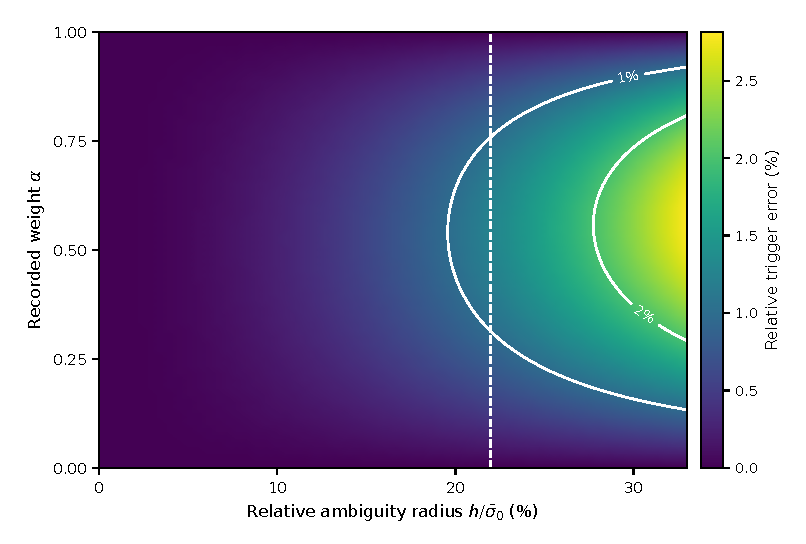
\includegraphics[width=\columnwidth]{figures/fig3_error_map.pdf}
\caption{Relative trigger error of the affine rule against the numerically computed $\aMEU$ benchmark. The grid covers ambiguity radius $h/\sbar$ and recorded weight $\alpha$ at the baseline calibration and $V_0=I$. Shading shows the relative trigger error in percent. White contours mark the 1\% and 2\% levels. The dashed vertical line marks $h/\sbar=22\%$, the upper bound of the primary radius range. The error peaked near $\alpha=1/2$ and vanished at the endpoint weights, consistent with Proposition~\ref{prop:accuracy}(ii).}
\label{fig:errormap}
\end{figure}
